\documentclass[pdf,color]{UoBnote}
\usepackage{epstopdf}
\usepackage{float}
\usepackage{amsmath}
\author{Samuel Delacruz\\
				sjd054@bham.ac.uk\\
				1090154}

\shorttitle{}
\title{Computational Modelling of Physical Systems\\Worksheet 3}
\date{\today}
\issue{3}

\begin{document}


\iffalse
	\em{TO DO:}
		
\fi

\maketitle
\tableofcontents
\listoffigures
\listoftables
\vspace{1cm}\hrule \vspace{1cm}
\newpage

\section{Introduction}
In this assignment, methods of integrating ordinary differential equations will be explored.\\\\
Firstly, Euler's method will be explained and applied to a basic problem. The errors associated with the method will be discussed.\\\\
Following this, the Runge-Kutta method will be described, and used to solve a problem, using second-order and fourth-order Runge-Kutta algorithms. The respective results will be compared, and errors discussed.
\section{Euler's Method}
	\subsection{Theory}
	Euler's method is a basic, but inefficient method of numerical approximation of differential equations.\\
	It is described as such, when considering a general first order differential equation,
	
	\begin{equation}\label{eq:basic_ode}
	\frac{dy}{dx}(x) = f(x,y)
	\end{equation}
	
	Can also be written as,
	
	\begin{equation}
	\frac{dy}{dx}(x) = \lim\limits_{h\rightarrow0}\frac{y(x+h)-y(x)}{h}
	\end{equation}
	
	This leads to the definitions of $y_0 = y(x_0)$ and $y_1 = y(x_0 + h)$.
	
	Expanding $y_1$ as a series gives,
	
	\begin{equation}
	y_1 = y(x_0) + y'(x_0)h + \frac{1}{2}y''(x_0)h^2 + ...
	\end{equation}
	
	Omitting powers of $h^3$ and above. Referring to equation (\ref{eq:basic_ode}), we can see that this may be re-written as,
	
	\begin{equation}
	y_1 = y(x_0) + hf(x_0,y_0) + O(h^2)
	\end{equation}
	
	So we can see that the error in using one step of Euler's method is of $O(h^2)$.\\\\
	However, for a good numerical approximation of the solution to a differential equation, we should aim for a set of values for many values of our dependent variable.\\\\
	Hence, if we apply the method $n$ times in succession, we will have,
	
	\begin{equation}
	y_n = y(x_0) + nhf(x_0,y_0) + O(nh^2)
	\end{equation}
	
	But, $n \propto h^{-1}$, so the $O(nh^2)$ term becomes $O(h)$. This means that the error expected from implementations of Euler's method is of $O(h)$, and will be investigated.
	\subsection{Procedure}
	To demonstrate Euler's method, a C++ program can be written to solve the differential equation
	
	\begin{equation}
	\frac{dy}{dt} = 1 + y^2 ,
	\end{equation}
				
	with initial condition $y(0) = 0$, for $y(\pi/4)$.\\\\
	This equation has the solution
	
	\begin{equation}
	y(t) = \tan(t)
	\end{equation}
	
	So $y(\pi/4) = \mathbf{1}$. This value will be used as a reference value, to compare to computed values at different values  of $h$.\\\\
	
	A program, named "euler.cpp" has been written to solve the described problem, and may be compiled using G++, and run with the terminal command:\\
	\texttt{./euler.o [n] [filename]}\\
	Where [n] is the maximum number of intervals to use, and [filename] is the name of the file to save results to. \textbf{Warning: ensure that [filename] is unique, or risk overwriting previous results}. 
				
	\subsection{Results}
				
				
				\begin{figure}[H]
					\centering
						\fbox{
						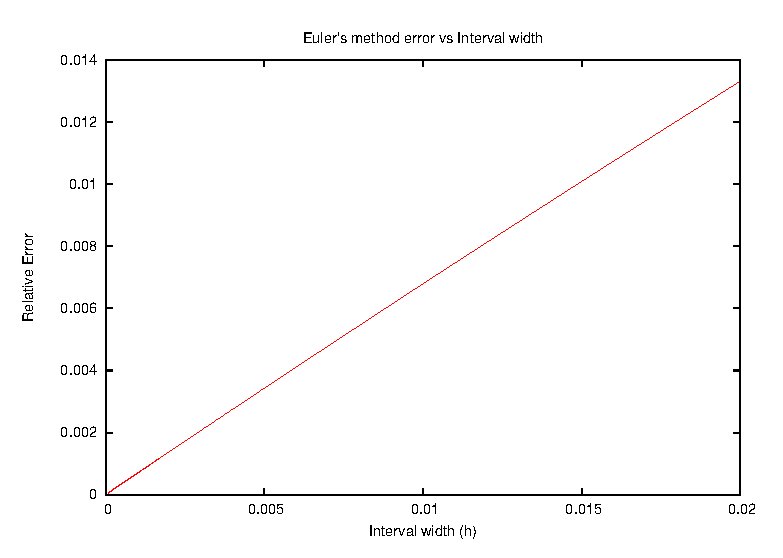
\includegraphics{figures/euler-h-vs-e.eps}}
					\caption{Plot of Euler's method relative error vs interval width}
					\label{fig:eu-e-vs-h-1}
				\end{figure}
	Figure (\ref{fig:eu-e-vs-h-1}) shows the evolution of errors in the program written as $h$ increases. As expected, the error in the approximate solution is $O(h)$, as demonstrated by the straight line on a linear scale graph.\\
	Even when using $n=10000$, the value for $y(\pi/4)$ is calculated as $9.999455690423819\cdot10^{-1}$, which has a relative error $\epsilon = 5.443095761814565\cdot10^{-5}$. This confirms that relative error is $O(h)$, or alternatively $O(n^{-1})$.\\\\
	Clearly, Euler's method is inefficient at solving this particular problem, and more efficient algorithms must be explored which have faster convergence.
		
\section{The Runge-Kutta method}
	\subsection{Theory}
	The Runge-Kutta method improves upon Euler's method by averaging the slope of the function between $x$ and $x + h$. In the second order Runge Kutta method, the value of the slope at the midpoint of the interval is used to reach the end of the interval from the beginning. This results in a closer fitting to the curve, generating an overall relative error $O(h^3)$. This method is therefore far more efficient than the basic Euler's method.\\
	\\
	For solving systems of first order differential equations, using the second-order Runge-Kutta method, the following procedure applies
	
	\begin{align}
	\mathbf{k}_1 & = h\mathbf{f}(x_n,\mathbf{y}_n)\\
	\mathbf{k}_2 & = h\mathbf{f}(x_n + \frac{h}{2},\mathbf{y}_n + \frac{\mathbf{k}_1}{2})\\
	\mathbf{y}_{n+1} & = \mathbf{y}_n + \mathbf{k}_2 + O(h^3)
\end{align}		
	
	To put this into practice, another problem shall be solved. In this case, the Simple Harmonic Oscillator will be considered, with unit mass and potential
	
	\begin{equation}
	V(x) = \frac{1}{2}x^2
	\end{equation}
	
	The Simple Harmonic Oscillator with unit mass can be described by
	
	\begin{align}
	F &= \frac{d^{2}x}{dt^2}\\
		&= -x
	\end{align}
	
	Which may be decomposed into a system of two coupled  first order equations
	
	\begin{align}
	\frac{dx}{dt} & = p\\
	\frac{dp}{dt} & = -x
	\end{align}
	
	These equations can be solved together using the Runge-Kutta method as described previously, and they have an analytical solution of
	
	\begin{align}
	x(t) = x_0\cos(t)
	\end{align}
	
	\subsection{Procedure}
	
	\subsection{Results}
	
	
			
\section{Appendices}

	\subsection{Tables of Data}
		\subsubsection{Euler's Method Data}
		
			\begin{table}[H]
			\centering
			\fbox{
    \begin{tabular}{l|l|l}
    \textbf{Intervals (n)} & \textbf{Approximation (y)} & \textbf{Relative Error (E)}\\
    \hline
    1     & 7.853981633974483e-01 & 2.146018366025517e-01 \\
    2     & 8.459572975386589e-01 & 1.540427024613411e-01 \\
    3     & 8.801189879195483e-01 & 1.198810120804517e-01 \\
    4     & 9.018822813149980e-01 & 9.811771868500196e-02 \\
    5     & 9.169419341833210e-01 & 8.305806581667896e-02 \\
    6     & 9.279826868386274e-01 & 7.201731316137261e-02 \\
    7     & 9.364257661502460e-01 & 6.357423384975402e-02 \\
    8     & 9.430927338362762e-01 & 5.690726616372377e-02 \\
    9     & 9.484914877726021e-01 & 5.150851222739794e-02 \\
    10    & 9.529529514142623e-01 & 4.704704858573772e-02 \\
    11    & 9.567020195541525e-01 & 4.329798044584754e-02 \\
    12    & 9.598969005441126e-01 & 4.010309945588741e-02 \\
    13    & 9.626521443407428e-01 & 3.734785565925725e-02 \\
    14    & 9.650527402357407e-01 & 3.494725976425928e-02 \\
    15    & 9.671630805568465e-01 & 3.283691944315348e-02 \\
    16    & 9.690328475730891e-01 & 3.096715242691095e-02 \\
    17    & 9.707009895207200e-01 & 2.929901047927996e-02 \\
    18    & 9.721984725322474e-01 & 2.780152746775255e-02 \\
    19    & 9.735502268486828e-01 & 2.644977315131725e-02 \\
    20    & 9.747765498288290e-01 & 2.522345017117100e-02 \\
    21    & 9.758941348377806e-01 & 2.410586516221935e-02 \\
    22    & 9.769168374909493e-01 & 2.308316250905074e-02 \\
    23    & 9.778562543070635e-01 & 2.214374569293653e-02 \\
    24    & 9.787221652667678e-01 & 2.127783473323219e-02 \\
    9995  & 9.999455418176355e-01 & 5.445818236449185e-05 \\
    9996  & 9.999455472647586e-01 & 5.445273524140593e-05 \\
    9997  & 9.999455527107965e-01 & 5.444728920345199e-05 \\
    9998  & 9.999455581557488e-01 & 5.444184425118515e-05 \\
    9999  & 9.999455635996066e-01 & 5.443640039337616e-05 \\
    10000 & 9.999455690423819e-01 & 5.443095761814565e-05 \\
    \end{tabular}}
\end{table}


\end{document}
